
\documentclass[10pt]{article}
\usepackage{amssymb,amsmath,amsthm,amsfonts}
\usepackage{multicol,multirow}
\usepackage{ifthen}
\usepackage{amsmath}
\usepackage{physics}
\usepackage{geometry}
\usepackage{tikz}

\newcommand*\oiint{%
  \vcenter{\hbox{%
    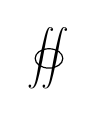
\begin{tikzpicture}[baseline=(A.base)]
      \node[inner sep=0pt] (A) {$\displaystyle\int\mspace{-12mu}\int$};
      \draw[line width=0.1ex] ([xshift=0.02em]A.center) ellipse (0.5em and 0.35em); 
    \end{tikzpicture}%
  }}%
}

\ifthenelse{\lengthtest { \paperwidth = 11in}}
    { \geometry{top=.5in,left=.5in,right=.5in,bottom=.5in} }
	{\ifthenelse{ \lengthtest{ \paperwidth = 297mm}}
		{\geometry{top=1cm,left=1cm,right=1cm,bottom=1cm} }
		{\geometry{top=1cm,left=1cm,right=1cm,bottom=1cm} }
	}
\pagestyle{empty}
\makeatletter
\renewcommand{\section}{\@startsection{section}{1}{0mm}%
    {-1ex plus -.5ex minus -.2ex}%
        {0.5ex plus .2ex}%x
            {\normalfont\large\bfseries}}
\renewcommand{\subsection}{\@startsection{subsection}{2}{0mm}%
    {-1explus -.5ex minus -.2ex}%
        {0.5ex plus .2ex}%
        {\normalfont\normalsize\bfseries}}
\renewcommand{\subsubsection}{\@startsection{subsubsection}{3}{0mm}%
    {-1ex plus -.5ex minus -.2ex}%
        {1ex plus .2ex}%
            {\normalfont\small\bfseries}}
            
\makeatother
\setcounter{secnumdepth}{0}
\setlength{\parindent}{0pt}
\setlength{\parskip}{0pt plus 0.5ex}

\begin{document}

\raggedright




\setlength{\columnseprule}{0.4pt}
\begin{multicols}{2}
\setlength{\premulticols}{1pt}
\setlength{\postmulticols}{1pt}
\setlength{\multicolsep}{1pt}
\setlength{\columnsep}{2pt}

\large{\textbf{UBC MATH 264: Vector Calculus for Electrical Engineering}} \\
\normalsize
\subsection*{Vector Identities}

For vectors $\vb{u} = \langle u_x,u_y,u_z\rangle, \vb{v} = \langle v_x,v_y,v_z\rangle, \vb{w} = \langle w_x,w_y,w_z\rangle$,\\[4pt]

Unit Vector \hfill $\displaystyle \hat{u}= \frac{\vb{u}}{||\vb{u}||}\qquad\qquad\qquad\qquad\qquad\qquad\qquad\quad$\\[4pt]

Dot Product \hfill $\vb{u} \cdot \vb{v} = u_xv_x + u_yv_y + u_zv_z = ||\vb{u}||\,||\vb{v}||\cos\theta$\\[4pt]

Magnitude \hfill$||\vb{u}|| = \sqrt{\vb{u}\cdot\vb{u}} = \sqrt{u_x^2 + u_y^2 + u_z^2}\qquad\qquad\quad\,$\\[4pt]

Cross Product \hfill$\displaystyle \vb{u} \times \vb{v} = \begin{vmatrix}
 \vb{a}_x & \vb{a}_y & \vb{a}_z\\
 u_x & u_y & u_z\\
 v_x & v_y & v_z
\end{vmatrix}\qquad\qquad\qquad\qquad\quad\,$\\[4pt]

Projection\hfill $\text{proj}_{\vb{u}}(\vb{F}) = \displaystyle\left(\frac{\vb{F} \cdot \vb{u}}{\vb{u} \cdot \vb{u}}\right)\vb{u}\qquad\qquad\qquad\qquad\,\,\,\,$


\subsection*{Parameterization}
Arc Length \hfill$\displaystyle \int_C\dd s=\int_{a}^{b} ||\vb{r}'(t)||\, \dd t\qquad\qquad\qquad\qquad\quad\,$\\[4pt]

Surface Area \hfill$\displaystyle \iint_S \dd S=\iint\limits_D \left|\left|\vb{r}_{u}\times\vb{r}_{v}\right|\right| \,\dd u\,\dd v\qquad\qquad\quad\,\,\,$\\[4pt]

Line Integral\hfill$\displaystyle \int_C \vb{F} \cdot \dd \vb{r} = \int_a^b \vb{F}(\vb{r}(t)) \cdot \vb{r}'(t)\, \dd t\qquad\qquad\quad\,\,$\\[8pt]

Surface Integral\hfill$\displaystyle \iint \limits_S\vb{F}\cdot \dd\vb{S}=\iint
\limits_D \vb{F}(\vb{r}(u,v))\cdot \left(\vb{r}_{u}\times\vb{r}_v\right)\dd u\,\dd v$

\normalsize


\normalsize

\subsection*{Cartesian Coordinates $(x,y,z)$}

Line Element \hfill $\dd \vb{l} = \vb{a}_x\dd x+\vb{a}_y\dd y+\vb{a}_z\dd z\qquad \quad\quad\,\,\,$\\[4pt]

Volume Element \hfill $\dd V = \dd x\,\dd y\,\dd z\qquad \qquad\qquad\qquad\quad\,$\\[4pt]

Gradient \hfill $\displaystyle \nabla f = \pdv{f}{x}\mathbf{a}_x+\pdv{f}{y}\mathbf{a}_y+\pdv{f}{z}\mathbf{a}_z\quad\quad\,\,\,\,\,$\\[4pt]

Curl \hfill$\displaystyle \nabla \times \vb{F} =  \begin{vmatrix}
 \vb{a}_x & \vb{a}_y & \vb{a}_z\\[3pt]
 \pdv{x} & \pdv{y} & \pdv{z}\\[3pt]
  F_{x} & F_{y} & F_{z}
\end{vmatrix}\qquad\qquad\quad\,$\\[4pt]

Divergence \hfill$\displaystyle \nabla \cdot \vb{F} = \pdv{F_x}{x}+\pdv{F_y}{y}+\pdv{F_z}{z}\qquad\quad\,\,\, $\\[4pt]

\subsection*{Cylindrical Coordinates $(\rho,\phi,z)$}

Transformation\qquad$x=\rho \cos \phi,\quad y = \rho \sin \phi,\quad z=z$\\[4pt]

Local Basis\hfill $\vb{a}_\rho = \cos \phi \,\vb{a}_x + \sin\phi\,\vb{a}_y\qquad\quad\qquad\,$\\[4pt]

\hfill$\vb{a}_\phi = -\sin \phi \,\vb{a}_x + \cos\phi\,\vb{a}_y\qquad\qquad\,$\\[4pt]

Line Element\hfill$\dd \vb{l} = \vb{a}_\rho\dd \rho+\rho\vb{a}_\phi\dd \phi+\vb{a}_z\dd z\quad\qquad\,\,\,\,\,$\\[4pt]

Volume Element \hfill$\dd V = \rho\,\dd \rho\,\dd \phi\,\dd z\qquad\qquad\qquad\qquad\,\,$\\[4pt]

Gradient \hfill$\displaystyle \nabla f = \pdv{f}{\rho}\mathbf{a}_\rho+\frac{1}{\rho}\pdv{f}{\phi}\mathbf{a}_\phi+\pdv{f}{z}\mathbf{a}_z\qquad$

Curl\hfill $\displaystyle \nabla \times \vb{F} =  \frac{1}{\rho}\begin{vmatrix}
 \vb{a}_\rho & \rho\vb{a}_\phi & \vb{a}_z\\[3pt]
 \pdv{\rho} & \pdv{\phi} & \pdv{z}\\[3pt]
  F_{\rho} & \rho F_{\phi} & F_{z}
\end{vmatrix}\qquad\quad\,\,\,\,\,$\\[4pt]

Divergence\hfill$\displaystyle\nabla \cdot \vb{F} = \frac{1}{\rho}\pdv{\rho}(\rho F_\rho)+\frac{1}{\rho}\pdv{F_\phi}{\phi}+\pdv{F_z}{z}\,$

\subsection*{Spherical Coordinates $(r,\theta,\phi)$}

Transformation\quad $x=r\sin \theta \cos \phi,\ y = r\sin \theta\sin \phi,\ z = r\cos \theta$\\[4pt]

Local Basis \hfill$\vb{a}_r = \sin\theta\cos \phi \,\vb{a}_x + \sin\theta\sin\phi\,\vb{a}_y+\cos\theta \,\vb{a}_z$\\[4pt]
\hfill$\vb{a}_\theta = \cos \theta\cos \phi \,\vb{a}_x + \cos\theta\sin\phi\,\vb{a}_y-\sin\theta \,\vb{a}_z$\\[4pt]
\hfill$\vb{a}_\phi = -\sin\phi\, \vb{a}_x + \cos\phi\, \vb{a}_y\qquad\qquad\qquad\quad\,\,\,\,$\\[4pt]

Line Element \hfill$\dd \vb{l} = \vb{a}_r\dd r+r\vb{a}_\theta\dd \theta+r\sin \theta\,\vb{a}_\phi\dd \phi\qquad\qquad\,\,\,\,$\\[4pt]

Volume Element \hfill$\dd V = r^2\sin\theta \,\dd r\,\dd\theta \,\dd \phi\qquad\qquad\qquad\qquad\quad\,\,$\\[4pt]

Gradient \hfill$\displaystyle \nabla f = \pdv{f}{r}\mathbf{a}_r+\frac{1}{r}\pdv{f}{\theta}\mathbf{a}_\theta+\frac{1}{r\sin \theta}\pdv{f}{\phi}\mathbf{a}_\phi\qquad\,\,\,\,$\\[4pt]

Curl \hfill$\displaystyle\displaystyle \nabla \times \vb{F} =  \frac{1}{r^2\sin\theta}\begin{vmatrix}
 \vb{a}_r & r\vb{a}_\theta & r\sin\theta\vb{a}_\phi\\[3pt]
 \pdv{r} & \pdv{\theta} & \pdv{\phi}\\[3pt]
  F_{r} & rF_{\theta} & r\sin\theta F_{\phi}
\end{vmatrix}\qquad\,\,$\\[4pt]

Divergence 
\[\displaystyle\nabla \cdot \vb{F} = \frac{1}{r^2}\pdv{r}(r^2F_r)+\frac{1}{r\sin \theta}\left[\pdv{\theta}(F_\theta\sin\theta)+\pdv{F_\phi}{\phi}\right]\]

\subsection*{Fundamental Theorems of Calculus}

Gradient Theorem \hfill$\displaystyle \int_C \nabla f \cdot \dd \vb{r} = f(\vb{r}(b))-f(\vb{r}(a))\,\,$\\[4pt]

Divergence Theorem\hfill $\displaystyle \iiint_V (\nabla \cdot \vb{F})\, \dd V = \oiint_{\partial V} \vb{F} \cdot \dd \vb{S}$\\[4pt]

Stokes's Theorem \hfill$\displaystyle \oint_C\vb{F} \cdot \dd \vb{r} = \iint_S (\nabla \times \vb{F}) \cdot \dd\vb{S}\quad\,\,\,\,$




\end{multicols}
\end{document}